\documentclass[conference]{IEEEtran}
\usepackage[left=15mm, right=15mm, bottom=10mm, top=10mm]{geometry}
\usepackage{cite}
\usepackage{subfigure}
\usepackage{amsmath,amssymb,amsfonts}
\usepackage{algorithmic}
\usepackage{graphicx}
\usepackage{textcomp}
\usepackage{xcolor}
\usepackage{relsize}
\usepackage{multirow}
\usepackage[plain,lined]{algorithm2e}
\usepackage{booktabs}
\def\BibTeX{{\rm B\kern-.05em{\sc i\kern-.025em b}\kern-.08em
    T\kern-.1667em\lower.7ex\hbox{E}\kern-.125emX}}


\usepackage{hyperref}
\hypersetup{
%	pdfauthor = {AUTHOR_NAME},
%	pdftitle = {TITLE},
%	pdfsubject = {PROJECT},
	% ***** Authors need to modify keyword by themselves! *****
%	pdfkeywords = {KEY_WORD1, KEY_WORD2},
	pdfcreator = {LaTeX with hyperref package},
	pdfproducer = {pdflatex} 
	pdfborder={0 0 0},
	linkcolor = blue,
	citecolor = blue,
	urlcolor = blue,
	colorlinks = true
}
\renewcommand\IEEEkeywordsname{Keywords}
\usepackage{tikz}
\usetikzlibrary{shapes.geometric, arrows}

\begin{document}

\title{[EST Checkpoint 3] HANDIO: A Wireless Hand Gesture Recognizer
Based on Muscle-Tension and Inertial Sensing}
\author{
\IEEEauthorblockN{Mew}
\IEEEauthorblockA{Department of Computer Science \\
National Tsing Hua University, Hsinchu City, Taiwan\\
Mew@est}
\and
\IEEEauthorblockN{Jun Luan, Ting-Chou Chien, Seungjae Lee, and Pai H. Chou}
\IEEEauthorblockA{
	\textit{Center for Embedded Cyber-Physical Systems,} \\
	\textit{ University of California, Irvine, CA 92697-2625 USA} \\
	\{jluan1, tchien, leesj3, phchou\}@uci.edu\\
}

}

\maketitle
\begin{abstract}
This paper describes a miniature, wearable wireless
hand-gesture recognition (HGR) system called HANDIO. It ob-
tains its input from not only traditional inertial sensors but also
a muscle tension sensor (MTS). The addition of MTS enables
recognition of a much broader range of intuitive hand gestures,
particularly those involving the wrist, that would otherwise
be difficult to distinguish by traditional inertial-only HGRs.
Among MTSs, we choose an optical MTS over the conventional
surface electromyography (sEMG) for the small size, low power
consumption, wearing comfort, and good detection rate. This
novel miniaturized design enables the whole system to be easily
patched on the wrist area or integrated into a wearable device
such as a wristband or watch without extra wiring. Experimental
results show that a total of 8 hand gestures involving the wrist can
be recognized with a detection rate over 93$\%$. The average power
consumption of the optical sensor is only around 258$\mu$W. This
versatile system can also be used to detect other joint activities
such as the elbow and knee joint.
\end{abstract}

\begin{IEEEkeywords}
Optical sensors, Accelerometers, Sensor fusion,
Wireless sensor networks
\end{IEEEkeywords}
\section{Introduction}
Hand gesture recognition has drawn increasingly interest
for numerous human-computer interface (HCI) applications
such as gaming control, aged or disabled care, sports fitness,
etc. Some early systems explored technologies such as com-
puter vision and capacitive sensor \cite{c1,c2,c3}, but their bulkiness
has limited their use to controlled environments \cite{c4} such
as research labs or hospitals. The emergence of low-power,
miniature hardware components with sensing, computation,
and communication capabilities has made possible a new
generation of a wireless devices such as a wrist watch \cite{c5},
wristband \cite{c6}, or smartphone, making ubiquitous computing a
reality.
\subsection{Sensing Technologies}
Most wearable HGRs to date perform inertial sensing (i.e.,
acceleration and rotation) as the primary modality for acquiring
gesture data. One reason is that accelerometers (ACC) and
gyroscopes are widely available in small sizes and in low
power. However, they are limited to detecting the trajectory
of the whole hand or forearm, such as drawing a circle or a
square, but fail to differentiate the different wrist activities.
Many commonly used hand gestures involve the movement of
the wrist. One example is that a hand-up gesture for ``stop``
generates nearly the same signal as a slight forearm shaking
but with smaller acceleration values in all three axes. Other
gestures may include a hand swing of directions, making a
fist, etc. These gestures are natural to users but can be difficult
to detect by an ACC.

\begin{figure}[t]
\centering
\includegraphics[width=8cm]{fig/fig1}
\caption{Proposed hardware system. Top left: optical sensor
board, top right: BLE and MPU-9250 board, bottom: battery.}
\end{figure}


Muscle tension can be sensed by surface electromyography
(sEMG) or optical muscle tension sensing (OMTS). The former
is most widely used but has not been amenable to wearable
HGRs. It requires a minimum of two electrodes, i.e., plus and
minus, to extract the differential signal generated by muscle
contraction. Many applications require three with an extra
ground electrode serving as a reference for the instrumentation
amplifier \cite{c7}. Commercial electrodes have to be wired and are
usually about 30 mm in diameter \cite{c8}. The ground electrode
is critical to the performance and has to be placed far away
from the target muscle to generate a stable reference. As an
alternative, we explore optical sensors similar to those used
in pulse oximeters for detecting oxygen concentration level
(SpO2) \cite{c9} and heart rate. It uses an LED to emit light into
human tissue and a PD to detect the reflected optical signal.
We validate the effectiveness of OMTS in terms of size, power
consumption, and wearing comfort.
\subsection{Proposed HANDIO System}
In this paper, we present HANDIO, for HAND gesture recognizer
based on Inertial and Optical muscle-tension sensing.
It consists of both the wearable hardware and the data-fusion
algorithm.

1) Hardware: The HANDIO hardware consists of an
OMTS, a triaxial accelerometer, and a Bluetooth Low Energy
(BLE) system-on-chip (SoC). The optical subsystem can be
made very small and lightweight by using an LED-PD combo
chip \cite{c10}. The overall dimension of the whole prototype system
is only 30 mm (L) $\times$ 15 mm (W) $\times$ 8 mm (H) with the largest
part being the 90 mAh lithium battery, as shown in Fig. 1, and
a production version can be made significantly more compact.
This novel miniaturized design enables the whole system to be
easily patched on the wrist area or integrated into a wristband
or watch without any extra sensor or wire.

To reduce the system power, the LED is controlled by fast switching pulse width modulation (PWM) signal. Our
experimental result also shows that the optical MTS is free
from baseline wondering and motion artifact. This feature
avoids the heavyweight filtering process and complicated pattern
recognition algorithms, thus further saving the system
power.

2) Fusion Algorithm: We also propose a fusion algorithm,
which includes rapid optical signal induced segmentation,
Dynamic Time Warp (DTW) \cite{c11}, and decision fusion. The
fusion of optical and acceleration data increases the recognizable
gestures. We tested a total of 8 wrist-involved hand
gestures with a detection rate over 93$\%$. The average power
consumption of the optical sensor is 258$\mu$W, which is only
0.4$\%$ of the overall system power.

The contribution of this work lies in the novel hardware
sensing platform design and the fusion algorithm. Even though
this work focuses only on the HGR, this system is also versatile
enough for detecting other joint or muscle activities such as
elbows and knees movement.
\subsection{Paper Outline}
This paper first provides a background on the OMTS sensor
and accelerometer-based hand gesture recognition systems. We
then describe the proposed sensing system and sensor-fusion
algorithm. Experimental results are analyzed with a discussion
of the implications. We also demonstrate the versatility of
the system by applying it to other joint movement detection.
Finally, we conclude with a summary and future works.
\section{BACKGROUND AND RELATED WORKS}
Single ACC-based hand gesture recognition has been well
studied. One advantage of ACC is its availability on many
off-the-shelf portable devices. Examples include TI Chronos
Watch \cite{c5}, Nintendo Wii remote controller, and virtually all
smartphones. A digital ACC consumes less than 1 mW in
active mode. Acceleration data can be easily processed locally
or transferred through the wireless interface. On the software
side, simple filters such as low-pass filter (LPF) or median
filter \cite{c12} are usually used to smooth the signal before using
either feature-based or template-based detection algorithms to
detect a gesture. Feature-based methods use machine-learning
techniques such as Hidden Markov Model (HMM) or Support
Vector Machine (SVM) \cite{c3} to classify the signal according
to the extracted features. High accuracy is reported \cite{c13} but
a large training set is required to ensure high detection rate.
In template recognition, a widely used technique is dynamic
time warping (DTW). It can get started with only one template
for each gesture \cite{c14}. The signal is usually divided into fixedlength
segments, and dynamic programming is used to find

\tikzstyle{startstop} = [rectangle, rounded corners, minimum width=1cm, minimum height=1cm,text centered, draw=black, fill=red!30]

\tikzstyle{process} = [rectangle, minimum width=1cm, minimum height=1cm, text centered, text width=1cm, draw=black, fill=orange!30]

\tikzstyle{decision} = [diamond, minimum width=0.5cm, minimum height=0.5cm, text centered, text width=0.5cm, draw=black, fill=green!30]

\tikzstyle{arrow} = [thick,->,>=stealth]


\begin{tikzpicture}[node distance=1.8cm]
\node (start) [startstop] {\fontsize{8}{4}\selectfont Start};
\node (pro1) [process, right of=start] {\fontsize{5}{4}\selectfont Preprocessing \\ (ACC+MTS)};
\node (pro2) [process, right of=pro1] {\fontsize{5}{4}\selectfont Segmentation \\ (MTS Only)};
\node (dec1) [decision, right of=pro2] {\fontsize{3}{4}\selectfont Length \\ Checking};
\node (pro3) [process, below of=pro1] {\fontsize{5}{4}\selectfont Rejection};
\node (pro4) [process, below of=pro3] {\fontsize{5}{4}\selectfont Decision \\ Fusion};
\node (pro5) [process, right of=pro4] {\fontsize{5}{4}\selectfont 3D ACC DWT};
\node (dec2) [decision, right of=pro5] {\fontsize{3}{4}\selectfont Score$\tiny<$THD\_S};
\node (pro6) [process, right of=dec2] {\fontsize{5}{4}\selectfont 1D MTS DWT};
\node (stop) [startstop, left of=pro4] {\fontsize{8}{4}\selectfont End};
\draw [arrow] (start) -- (pro1);
\draw [arrow] (pro1) -- (pro2);
\draw [arrow] (pro2) -- (dec1);
\draw [arrow] (dec1) -| node[anchor=east] {YES} (pro6);
\draw [arrow] (dec1) |- node[anchor=south] {NO} (pro3);
\draw [arrow] (dec2) -- node {YES} (pro5);
\draw  (dec1) -- (dec2);
\draw [arrow] (pro6) -- (dec2);
\draw [arrow] (pro5) -- (pro4);
\draw [arrow] (pro3) -| (stop);
\draw [arrow] (pro4) -- (stop);
\end{tikzpicture}

\begin{figure}[h]
\centering
\caption{Detection Algorithm}
\end{figure}

the best matching subsequence with the preset templates. The
complexity of DTW is O(pST) with S being the segment size,
T the template size, and p the number of preset templates.
It can be easily implemented on a mobile platform such as a
smartphone and many modern microcontroller units (MCU).

To overcome the limitations of single ACC-based systems’
inability to detect wrist movements, multiple previous works
suggest to couple sEMG with ACC. In \cite{c15}, \cite{c16}, HMM, Kmeans
clustering, and decision fusion are used to fuse the
multi-channel sEMG signal with ACC. A set of more than
18 gestures can be detected with a detection rate of over
90$\%$. However, a multi-channel sEMG needs to be wired,
and electrodes are big in size and can be uncomfortable to
wear. Most applications require an extra troublesome step of
skin preparation \cite{c8}, which generally includes hair removal,
cleaning the skin, and applying conductive gel. The gel may
cause skin irritation and also introduces instability as the
gel dries over the time, thereby causing degradation of the
signal quality and baseline wondering. The closest one to our
system is \cite{c17}, which uses a single-channel sEMG with three
electrodes 30 mm in diameter. The muscle contraction signal
from sEMG is used as on-off control and only five gestures
can be detected. It is made wearable with a much smaller size
than the other two but still an order of magnitude larger than
our proposed system and cannot solve the electrode problem.
Therefore, ACC-sEMG-based systems are only suitable for a
controlled environment.

New sensing technologies, especially low-power wearable
sensors, provide potential solutions to this problem. Optical
sensor-based MTS is very promising in replacing sEMG in
this application due its size and wearing comfort. A wellknown
application of optical sensor is pulse oximetry, which
is acquired from an LED-PD pair. The LED emits light into
human tissue while the PD measures the transmittance or
reflectance of light. When used for muscle tension, only the
reflectance can be measured. It is a fairly complicated process
since the muscle movement has a triple effect: the muscle fiber
contraction changes both the light absorbance and the reflected
light path, while the blood volume in the muscle also affects
the reflected light. As a result, muscle movements manifest
as changes to the signal frequencies and amplitude in the PD
output. It is shown in \cite{c18} that optical sensors can differentiate
between isometric and isotonic contraction and in work \cite{c19},
\cite{c20}, similar optical sensors are used to monitor the upper
limb movement for controlling prosthetic limbs. In all these
works, the optical signal is only used for on-off control. Our
study shows that far more details are provided even in a singlechannel
MTS. We will show how to utilize the MTS signal in
template matching.
\section{TECHNICAL APPROACH}
We propose a recognition algorithm based on DTW and
decision fusion. The flowchart of the algorithm is shown in
Fig. 2.

\begin{figure}[t]
\centering
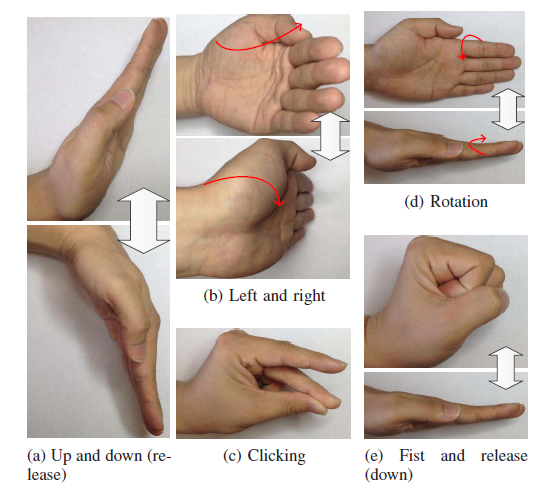
\includegraphics[width=8cm]{fig/fig3}
\caption{Gestures set. (No distinction between the down gesture
from the up position and the release gesture from the fist
position.)}
\end{figure}

\begin{figure}[t]
\centering
\includegraphics[width=8cm]{fig/fig4}
\caption{Filtered Signal}
\end{figure}

\subsection{Gesture Set}
Fig. 3 shows the tested gestures. What distinguishes them
from those that can be handled by previous ACC-based systems
\cite{c4}, \cite{c13}, \cite{c14} is their use of significant wrist movements,
such as hand up, clicking, and making a fist.

\subsection{Preprocessing and Segmentation}
In the preprocessing stage, a median filter is used for
both MTS and ACC to remove the high-frequency noise. A
high-pass filter (HPF) is then used to remove the gravity
factor in all three axes of ACC. After the filtering, only the
MTS signal is normalized to reduce the influence of signal
amplitude variation due to different speeds of performing the
same gesture. The raw and the filtered signals are shown in
Fig. 4.

Segmentation is based solely on the amplitude of the MTS
signal. A double-thresholding algorithm, as shown in Algorithm
1, runs point by point to divide the signal into segments.
Previous single ACC-based systems \cite{c13}, \cite{c14} usually use a
fixed-size sliding window with overlap to segment the signal.
The signal content within the window has to be checked
constantly to see if any valid gestures exist. Longer delay will
be caused by the fixed window size. By setting the starting
point and ending point in the signal of interest, our MTS-based
segmentation improves the system response time while
naturally rejecting some segments based on their length. Any
signal that is too short or too long will be automatically
discarded and will not go to the computationally complex
dynamic programming.

The algorithm keeps counting the samples across or below
the corresponding amplitude threshold. Based on a series of
counting conditions, the algorithm resets the counter or outputs
the starting and ending points of the given segment. Fig. 5
shows a segmented MTS signal with its starting and ending
points. This algorithm requires that the gestures be done
separately with enough resting interval. Otherwise, several
segments may be counted as one and may be discarded due to
oversize.

\begin{figure}[t]
\centering
\includegraphics[width=8cm]{fig/fig5}
\caption{Signal Segmentation}
\end{figure}

\subsection{Dynamic Time Warping Algorithm}
As shown in Fig. 2, DTW is the core algorithm of detection.
It is performed to both MTS and ACC signals. After
preprocessing and segmentation, MTS signal is first checked
with all stored templates using one-dimensional DTW. Only
those templates with sufficiently high scores can be sent to
the next step. If the segmented signal does not match any
pattern over the threshold, then it will be discarded. We find
this rejection step to be able to effectively reduce the number of
false-positive detections due to casual, unintended movement.
The basic DTW algorithm is shown in Algorithm 2.

DTW finds a match between two time sequences by dynamic
programming. The idea is to find the shortest path in the
cost matrix as shown in Fig. 6, where each cell represents the
similarity score between the two corresponding subsequences.
The distance between two MTS samples is just the absolute
value, while for 3D acceleration samples, the distance is
calculated based on Euclidean distance as in shown in Eq. (1).
The matched signals in all four dimensions are shown in Fig. 7.

\begin{tiny}
\begin{equation}
\sqrt{(ACCX_1 - ACCX_2)^2 + (ACCY_1 - ACCY_2)^2 + (ACCZ_1 - ACCZ_2)^2}
\end{equation}
\end{tiny}

Two constraints are implemented here: warping window
constraint and slope constraint \cite{c11}. Warping window constraint
(line 1) prevents one point from matching any point
too far away by setting global forbidden area, shown as the
gray cells in Fig. 6, to eliminate the path far off the diagonal.
The local slope constraint (line 2) avoids the alignment paths
that are too steep or too shallow as shown in Fig. 6. The
slope value along the optimal path from the starting point to
each cell is stored in separate slope matrices. When exceeding
the threshold, the path will be discarded along the way. The
slope matrix is updated on line 3. If the two sequences are too
different from each other, then the template sequence will be
automatically rejected before DTW.
\subsection{Decision Fusion}
The final matching score of the segmented signal to each
template is given by Formula (2). It is a weighted average
of both MTS and ACC scores with the weight $\gamma$ = 0.66. The
template with the best score is selected as the output gesture.

\begin{small}
\begin{equation}
score\_final = \gamma\cdot score\_ACC+(1-\gamma)\cdot score\_MTS
\end{equation}
\end{small}
\section{IMPLEMENTATION}

\begin{figure}[t]
\centering
\subfigure[Cost matrix and warping window constraint]
{
  \includegraphics[width=4cm, scale=1]{fig/fig6a}
}
\subfigure[Slope constraint]
{
  \includegraphics[width=4cm, scale=1]{fig/fig6b}
}
\caption{Dynamic Time Warping with Constraints}
\end{figure}

\begin{figure}[t]
\centering
\includegraphics[width=8cm]{fig/fig7}
\caption{Signal matched with Dynamic Time Warping}
\end{figure}

\begin{figure}[b]
\centering
\includegraphics[width=8cm]{fig/fig8}
\caption{Proposed hybrid system}
\end{figure}

Fig. 8 shows the block diagram of the proposed HGR
system. It consists of a light emitter with a current source,
a photo diode (PD) with an OpAMP, an inertial sensor, and
a Bluetooth Low Energy (BLE) system-on-chip (SoC). To
quickly validate our design, we implement our sensor board
using a commercially available pulse-sensor design \cite{c21} but
customize the board to our design. For the accelerometer and
BLE board, we designed a prototype as shown in Fig. 1. Both
boards are connected using jumpers. The overall dimension of
the system including the battery is 30 mm (L) $\times$ 15 mm (W) $\times$
8 mm (H). The optical sensor board for prototyping purpose
may appear bulky but can be shrunk easily by fabricating a
flexible PCB, as the optical sensors themselves are small. Even
without optimization, the whole system is lightweight and can
be easily adhered onto the wrist area or further integrated into
a wearable sensing platform such as a wrist band or a watch.
The sensing location of the optical sensor is shown in Fig. 9.

\begin{figure}[t]
\centering
\includegraphics[width=6cm]{fig/fig9}
\caption{Sensing location on the wrist area.}
\end{figure}

\subsection{Optical Subsystem}
In the optical subsystem, the LED is driven by a PWMcontrolled
current source \cite{c22} for brightness control. The
LED current is limited to 500$\mu$A to prevent the on-surge
current during fast switching. The color of the LED is green
with a peak wavelength of 515 nm, which matches the peak
wavelength of the PD response curve. This way, the PD
response is maximized, thus further reducing the system power
consumption. The green LED color is also proved to be more
robust to motion artifact than other colors \cite{c23}. The LED
on-time is set to approximately 200$\mu$s in every 16 ms by
PWM control as shown in Fig. 11. In response to the LED,
the PD outputs a current that flows through the load resistor
to generates the voltage signal. The low-pass filter removes
noise and motion artifact in the voltage signal, and the OpAMP
amplifies it for sampling by the on-chip ADC on the CC2541.

\subsection{Accelerometer}
We use MPU-9250 \cite{c24} as the ACC controlled by the SPI
interface of CC2541. MPU-9250 is actually a 9 degree-off-reedom
(9-DoF) inertial sensor consisting of a triaxial ACC,
gyroscope, and compass. We use only the ACC for this test
while the gyro and compass are reserved for future use. The
typical operating current of the gyroscope is 3.2 mA and
only around 450$\mu$A for the ACC. The compass takes around
280$\mu$A and can be helpful to gesture recognition but it is
susceptible to the disturbance of other magnetic materials in
the vicinity \cite{c25}.


\subsection{Bluetooth Low Energy SoC}
CC2541 from TI is an integrated MCU and radio frequency
transceiver SoC that runs TI’s BLE protocol stack
\cite{c26} and the application code on a single chip. Industrystandard
profiles such as GATT (for attribute access) and GAP
(for connection and discovery) are already implemented. The
HGR system works as a slave server while the mobile device
(smartphone) works as a master client. The BLE stack runs
on a low-overhead, non-emptive, event-driven task executive
called OSAL, which implements tasks as call-back functions.

The CC2541 MCU performs MTS sampling, ACC reading,
and data transmission over BLE. The MCU remains in lowpower
mode normally. On each timer rollover, the MCU wakes
up, reads its ADC for the MTS signal, and reads the ACC data
from SPI. After all the data is acquired and stored into a local
buffer, the MCU queues a sending event in the scheduler and
go to low-power mode 3 (LPM3) again, from which the MCU
can be waken by interrupts only. The sending event will cause
the queued data to be sent the mobile client. This process
repeats at a rate of 62.5 Hz.
\section{EVALUATION}
\subsection{Detection Accuracy}
We tested our HGR system on three subjects, two male
and one female. One important aspect of HGR is the noise
rejection. In real situations, gestures coexist with random
activities. These random activity should be rejected instead of
being recognized as a valid gesture. Otherwise, the system will
become hard to use due to many false positives. We collected
40 non-gesture noise patterns, including random hand or wrist
shake with both short and long wrist activities from each
subject. Another 40 samples of each gesture from each person
are also record. The total collection time is over 1 hour each.
The system is implemented on a laptop computer to repeatedly
study the data. The detection rate is defined in Eq. (3).

\begin{footnotesize}
\begin{equation}
Detection\_Rate = 1-\frac{True\_Negatives+False\_Positives}{Total\_Gestures}
\end{equation}
\end{footnotesize}

As shown in Table I, the detection rate is over 93$\%$ with the
highest over 95$\%$. We also implemented a single ACC-based
HGR with the sliding window algorithm. A threshold is set to
reject the noise based on the DTW score. The result clearly
indicates that our system is superior to single ACC-based
system in terms of noise rejection and detection accuracy.

The detailed result for each gesture is shown in Table II.
The detection rate is just the true positive rate, since no noise
gesture is involved. Even though for some gestures, ACConly
results in slightly higher detection rate than the fusion
method does, the fusion method helps improve the accuracy
of the majority at a very small cost. The overall result shows
the advantage of decision fusion over the single ACC-based
method. The same gesture is usually done multiple times with
different stopping points or angles to record multiple templates
for each gesture. This multi-template setting helps eliminate
ambiguity. Fig. 10 shows the influence of the weight $\gamma$ in
Eq. (2). The detection rates for all three people go beyond
93$\%$ when $\gamma$ = 66$\%$.

\subsection{Power Consumption}
The power consumption of the system is measured using a
current probe. The current values are integrated over a period
of 5 minutes to calculate the average power consumption.
Fig. 11 shows the periodic current signal of the optical sensor
board. Even though the LED takes around 500$\mu$A when
turned on, the duty of PWM is around 1.25$\%$. The optical
sensor consumes around 258$\mu$W on average. The majority
of the power is consumed by BLE communication sending
and receiving data. The average power consumption of the
CC2541 and MPU-9250 is around 57.5 mW. Thus, the power
consumption increased by the MTS is only around 0.4$\%$ of
the system power. The current system can last for more than 6
hours without recharging. Further optimization for future work
includes lowering the SoC`s Tx power, adjusting the sampling
rate, and enabling threshold detection in the accelerometer.

\subsection{Time Delay}
The recognition system has also been ported to an
iPhone4s. The measured computation delay is around 50 ms
in the worst case with an average of 14 ms. Even with an
expansion of around 30 gestures, the delay is under 100 ms.

\begin{figure}[b]
\centering
\includegraphics[width=8cm]{fig/fig10}
\caption{Decision Weight}
\end{figure}

\begin{table}
\centering
\caption{Total Detection Rate}
\begin{tabular}{|c|c|c|c|c|} 
\toprule
Det. Alg.                  & Sub.   & TN & FP & Dec. Rate  \\ 
\hline
\multirow{3}{*}{Acc + MTS} & Male 1 & 18 & 4  & 93.89\%    \\ 
\cline{2-5}
                           & Male 2 & 11 & 5  & 95.56\%    \\ 
\cline{2-5}
                           & Female & 18 & 3  & 94.17\%    \\ 
\hline
\multirow{3}{*}{Acc}       & Male   & 25 & 17 & 88.33\%    \\ 
\cline{2-5}
                           & Male 2 & 14 & 9  & 93.61\%    \\ 
\cline{2-5}
                           & Female & 31 & 7  & 89.44\%    \\
\bottomrule
\end{tabular}
\end{table}


\begin{table}
\centering
\caption{Detection Rate of Each Gesture}
\scriptsize
\begin{tabular}{|c|c|c|c|c|c|} 
\toprule
Sub.                                                                                     & Gesture        & Fusion Rate & Acc. Rate & Temp. & Length         \\ 
\hline
\multirow{9}{*}{\begin{tabular}[c]{@{}l@{}}Male 1\\$\gamma$ = 0.66 \end{tabular}}           & Up             & 92.5\%      & 87.5\%    & 4     & 240ms-928ms    \\ 
\cline{2-6}
                                                                                         & Dn/Rel.        & 90.0\%      & 60.0\%    & 6     & 304ms-1312ms   \\ 
\cline{2-6}
                                                                                         & Rot.$\leftarrow$  & 92.5\%      & 95.0\%    & 2     & 304ms-1120ms   \\ 
\cline{2-6}
                                                                                         & Rot.$\rightarrow$ & 90.0\%      & 90.0\%    & 2     & 288ms-1200ms   \\ 
\cline{2-6}
                                                                                         & Fist           & 97.5\%      & 67.5\%    & 2     & 448ms-1120ms   \\ 
\cline{2-6}
                                                                                         & Clicking       & 97.5\%      & 32.5\%    & 4     & 336ms-1040ms   \\ 
\cline{2-6}
                                                                                         & Left           & 95.0\%      & 92.5\%    & 1     & 480ms-1200ms   \\ 
\cline{2-6}
                                                                                         & Right          & 97.5\%      & 100.0\%   & 1     & 288ms-768ms    \\ 
\cline{2-6}
                                                                                         & Tol.           & 94.4\%      & 78.1\%    & 22    & 240ms-1312ms   \\ 
\hline
\multirow{9}{*}{\begin{tabular}[c]{@{}l@{}}Male 2\\$\gamma$ = 0.82 \end{tabular}} & Up             & 97.5\%      & 100.0\%   & 5     & 512ms-1408ms   \\ 
\cline{2-6}
                                                                                         & Dn/Rel.        & 92.5\%      & 95.0\%    & 5     & 480ms-1264ms   \\ 
\cline{2-6}
                                                                                         & Rot.$\leftarrow$  & 97.5\%      & 97.5\%    & 4     & 592ms-2880ms   \\ 
\cline{2-6}
                                                                                         & Rot.$\rightarrow$ & 100.0\%     & 100.0\%   & 4     & 560ms-2384ms   \\ 
\cline{2-6}
                                                                                         & Fist           & 97.5\%      & 67.5\%    & 1     & 656ms-1376ms   \\ 
\cline{2-6}
                                                                                         & Clicking       & 92.5\%      & 100.0\%   & 3     & 1072ms-1488ms  \\ 
\cline{2-6}
                                                                                         & Left           & 100.0\%     & 50.0\%    & 2     & 784ms-1040ms   \\ 
\cline{2-6}
                                                                                         & Right          & 95.0\%      & 45.0\%    & 2     & 672ms-1296ms   \\ 
\cline{2-6}
                                                                                         & Tol.           & 96.56\%     & 81.9\%    & 26    & 480ms-2880ms   \\ 
\hline
\multirow{9}{*}{\begin{tabular}[c]{@{}l@{}}Female\\$\gamma$ = 0.75 \end{tabular}}        & Up             & 97.5\%      & 100.0\%   & 4     & 784ms-1392ms   \\ 
\cline{2-6}
                                                                                         & Dn/Rel.        & 97.5\%      & 100.0\%   & 5     & 624ms-1424ms   \\ 
\cline{2-6}
                                                                                         & Rot.$\leftarrow$  & 92.5\%      & 82.5\%    & 2     & 1024ms-1840ms  \\ 
\cline{2-6}
                                                                                         & Rot.$\rightarrow$ & 92.5\%      & 90.0\%    & 2     & 1264ms-2544ms  \\ 
\cline{2-6}
                                                                                         & Fist           & 92.5\%      & 80.0\%    & 2     & 448ms-1408ms   \\ 
\cline{2-6}
                                                                                         & Clicking       & 90.0\%      & 80.0\%    & 3     & 688ms-2480ms   \\ 
\cline{2-6}
                                                                                         & Left           & 95.0\%      & 77.5\%    & 2     & 912ms-1488ms   \\ 
\cline{2-6}
                                                                                         & Right          & 90.0\%      & 80.0\%    & 1     & 912ms-1264ms   \\ 
\cline{2-6}
                                                                                         & Tol.           & 94.4\%      & 86.3\%    & 21    & 448ms-2544ms   \\
\bottomrule
\end{tabular}
\end{table}

\subsection{Other Applications}
We also tested the system on elbow and knee joints. The
sensing locations are shown in Fig. 12. Signal samples are
shown in Fig. 13. The degree of freedom of movement is
generally less than the wrist joint. The MTS signal can be
used to detect the muscle movement around the joint while
the ACC data provides the detailed movement, such as moving
direction, timing, etc. The fusion of both MTS and ACC can
be synergistic in classifying the movements.
\begin{figure}[t]
\centering
\subfigure[PWM and PD output. Green:PWM, pink: PD output]
{
  \includegraphics[width=4cm, scale=1]{fig/fig11a}
}
\subfigure[Current consumption. Green:PWM, yellow: optical sensor board current signal]
{
  \includegraphics[width=4cm, scale=1]{fig/fig11b}
}
\caption{LED control and current consumption.}
\end{figure}

\begin{figure}[t]
\centering
\subfigure[Knee]
{
  \includegraphics[height=4cm, scale=1]{fig/fig12a}
}
\subfigure[Elbow]
{
  \includegraphics[height=4cm, scale=1]{fig/fig12b}
}
\caption{Sensing locations on the knee and elbow.}
\end{figure}

\section{CONCLUSIONS}
In this paper, we have presented HANDIO, a wireless
hybrid hand gesture recognition system of OMTS and ACC.
Compared with previous works, the proposed system strikes
the most balance among gesture variety, wearability, and power
consumption. The OMTS enables the detection of wrist movements,
which greatly increases the total number of detectable
gestures of the current single ACC-based HSG.

In addition to the hardware, we also describe a DTW
and decision fusion-based detection algorithm, which shows
a high detection rate. By fusing the MTS and ACC signals,
the system response time is also significantly improved. We
also show that the same system can be used in many other
body-area sensor applications. Altogether we are building the
next-generation, highly wearable sensor networks for accurate
human movement monitoring and tracking.

\begin{figure}[t]
\centering
\includegraphics[width=8cm]{fig/fig13a}
\caption{Signals from the knee and elbow joint.}
\end{figure}

\section*{Acknowledgments}
This work was sponsored by the National Institute of
Health (NIH) STTR Phase II Grant 2R42HL112435-03. The
content is solely the responsibility of the authors and does not
necessarily represent the official views of the sponsors.

%\bibliographystyle{IEEEtran}
\bibliographystyle{unsrt}
\bibliography{citation}

\end{document}
